\renewcommand{\thesection}{\Roman{section}}
\titleformat{\section}
{\normalfont\bfseries}{PHẦN~\thesection.}{0.4em}{}
\newcolumntype{C}[1]{>{\centering\arraybackslash}p{#1}}
\newcolumntype{L}[1]{>{\raggedright\arraybackslash}p{#1}}
\begin{tabular}{C{5cm}C{11cm}}
	\textbf{TRUNG TÂM MANABIE}& \textbf{ĐỀ ÔN TẬP KIỂM TRA HỌC KÌ 2} \\
	\textbf{ĐỀ 02}& \textbf{Môn: VẬT LÝ}\\
	\textit{(Đề có 05 trang)}& \textit{Thời gian làm bài: 50 phút, không kể thời gian phát đề}
	
	\noindent\rule{4cm}{0.8pt} \\
\end{tabular}
\hdc{
	\section{}
	Mỗi câu trả lời đúng thí sinh được \textbf{0,25 điểm}.
	\begin{center}
		\begin{tabular}{|C{2.5cm}|C{4.0cm}|C{2.5cm}|C{4.0cm}|}
			\hline
			\thead{Câu} & \thead{Đáp án} & \thead{Câu} & \thead{Đáp án}\\
			\hline
			1 & D &  10 & B \\ 
			\hline
			2 & A &  11 & B \\ 
			\hline
			3 & D &  12 & A \\ 
			\hline
			4 & D &  13 & C \\ 
			\hline
			5 & A &  14 & D \\ 
			\hline
			6 & B &  15 & B \\ 
			\hline
			7 & C &  16 & C \\ 
			\hline
			8 & B &  17 & D \\ 
			\hline
			9 & C &  18 & A \\ 
			\hline
		\end{tabular}
	\end{center}
	\section{}
	Điểm tối đa của 01 câu hỏi là \textbf{1 điểm}.
	\begin{itemize}
		\item Thí sinh lựa chọn chính xác 01 ý trong 1 câu hỏi được \textbf{0,1} điểm.
		\item Thí sinh lựa chọn chính xác 02 ý trong 1 câu hỏi được \textbf{0,25} điểm.
		\item Thí sinh lựa chọn chính xác 03 ý trong 1 câu hỏi được \textbf{0,50} điểm.
		\item Thí sinh lựa chọn chính xác cả 04 ý trong 1 câu hỏi được \textbf{1} điểm.
	\end{itemize}
	\begin{center}
		\begin{tabular}{|C{1.0cm}|C{2.0cm}|C{3.0cm}|C{1.0cm}|C{2.0cm}|C{3.0cm}|}
			\hline
			\thead{Câu} & \thead{Lệnh hỏi} &\thead{Đáp án\\ (Đ/S)} &\thead{Câu} & \thead{Lệnh hỏi} &\thead{Đáp án\\ (Đ/S)}\\
			\hline
			\multirow{4}{*}{\textbf{1}}& a) & Đ & \multirow{4}{*}{\textbf{3}} & a) & S \\
			\cline{2-3}\cline{5-6}
			& b) & Đ &                             & b) & Đ \\
			\cline{2-3}\cline{5-6}
			& c) & S &                             & c) & Đ \\
			\cline{2-3}\cline{5-6}
			& d) & S &                             & d) & Đ \\
			\hline
			\multirow{4}{*}{\textbf{2}}& a) & S & \multirow{4}{*}{\textbf{4}} & a) & S \\
			\cline{2-3}\cline{5-6}
			& b) & S &                             & b) & Đ \\
			\cline{2-3}\cline{5-6}
			& c) & Đ &                             & c) & Đ \\
			\cline{2-3}\cline{5-6}
			& d) & Đ &                             & d) & S \\
			\hline		                           		                       
		\end{tabular}
	\end{center}
	\section{}
	Mỗi câu trả lời đúng thí sinh được \textbf{0,25 điểm}.
	\begin{center}
		\begin{tabular}{|C{2.5cm}|C{4.0cm}|C{2.5cm}|C{4.0cm}|}
			\hline
			\thead{Câu} & \thead{Đáp án} & \thead{Câu} & \thead{Đáp án}\\
			\hline
			1 & 5 &  4 & 0,23 \\ 
			\hline
			2 & 3,2 &  5 & 509250 \\ 
			\hline
			3 & A &  6 & 6\\ 
			\hline
		\end{tabular}
	\end{center}
	\newpage
}
\setcounter{section}{0}
\section{Câu trắc nghiệm nhiều phương án lựa chọn.}
\textit{Thí sinh trả lời từ câu 1 đến câu 18. Mỗi câu hỏi thí sinh chọn một phương án.}
\begin{enumerate}[label=\bfseries Câu \arabic*:]
	\item Hiệu điện thế hai đầu mạch ngoài được xác định bằng biểu thức
	\begin{mcq}(4)
		\item $U_\text{N}=\calE+Ir$.
		\item $U_\text{N}=Ir$.
		\item $U_\text{N}=I\left(R+r\right)$.
		\item $U_\text{N}=\calE-Ir$.
	\end{mcq}
\hideall{
\textbf{Đáp án D.}
}

\item Dòng điện trong kim loại là dòng chuyển động có hướng của
\begin{mcq}
	\item các electron tự do ngược chiều điện trường.
	\item các ion âm ngược chiều điện trường.
	\item các electron tự do cùng chiều điện trường.
	\item các ion dương cùng chiều điện trường.
\end{mcq}
\hideall{
\textbf{Đáp án A.}
}

\item Theo định luật Ohm toàn mạch thì cường độ dòng điện mạch chính
\begin{mcq}
	\item tỉ lệ nghịch với điện trở mạch ngoài.
	\item tỉ lệ nghịch với suất điện động của nguồn.
	\item tỉ lệ nghịch với điện trở trong của nguồn.
	\item tỉ lệ nghịch với tổng điện trở trong và điện trở mạch ngoài.
\end{mcq}
\hideall{
\textbf{Đáp án D.}
}

\item Đặt một điện tích $q$ tại điểm M trong điện trường có cường độ điện trường $\SI{5000}{\volt/\meter}$ thì lực điện tác dụng lên điện tích đó có độ lớn $\SI{0.01}{\newton}$ và ngược hướng với vector cường độ điện trường. Giá trị của $q$ là
\begin{mcq}(4)
	\item $\SI{-5E-6}{\coulomb}$.
	\item $\SI{2E-6}{\coulomb}$.
	\item $\SI{5E-6}{\coulomb}$.
	\item $\SI{-2E-6}{\coulomb}$.
\end{mcq}
\hideall{
\textbf{Đáp án D.}\\
Độ lớn của $q$:
$$\left|q\right|=\dfrac{F}{E}=\SI{2E-6}{\coulomb}.$$
Vì $\vec{F}\uparrow\downarrow\vec{E}$ nên $q<0\Rightarrow q=\SI{-2E-6}{\coulomb}.$
}

\item Trong thời gian $t$, điện lượng dịch chuyển qua tiết diện thẳng của dây là $q$. Cường độ dòng điện không đổi được tính bằng công thức
\begin{mcq}(4)
	\item $I=\dfrac{q}{t}$.
	\item $I=\dfrac{q^2}{t}$.
	\item $I=\dfrac{t}{q}$.
	\item $I=qt$.
\end{mcq}
\hideall{
\textbf{Đáp án A.}
}

\item Đối với mạch điện kín thì hiệu suất của nguồn điện không được tính bằng công thức
\begin{mcq}(2)
	\item $H=\dfrac{U}{E}\cdot\SI{100}{\percent}.$
	\item $H=\dfrac{r}{R+r}\cdot\SI{100}{\percent}.$
	\item $H=\dfrac{A_\text{có ích}}{A_\text{tp}}\cdot\SI{100}{\percent}$.
	\item $H=\dfrac{R}{R+r}\cdot\SI{100}{\percent}.$
\end{mcq}
\hideall{
\textbf{Đáp án B.}
}

\item Một quả cầu nhỏ mang điện tích $\SI{2E-9}{\coulomb}$ đặt trong không khí. Cường độ điện trường tại một điểm cách quả cầu $\SI{3}{\centi\meter}$ là
\begin{mcq}(4)
	\item $\SI{E4}{\volt/\meter}$.
	\item $\SI{6E4}{\volt/\meter}$.
	\item $\SI{2E4}{\volt/\meter}$.
	\item $\SI{2E5}{\volt/\meter}$.
\end{mcq}
\hideall{
\textbf{Đáp án C.}\\
Cường độ điện trường tại điểm cách quả cầu $\SI{3}{\centi\meter}$ là:
$$E=\dfrac{k\left|q\right|}{\varepsilon r^2}=\SI{2E4}{\volt/\meter}.$$
}

\item Cho đoạn mạch có điện trở không đổi. Nếu hiệu điện thế giữa hai đầu đoạn mạch tăng 3 lần trong cùng khoảng thời gian thì năng lượng điện tiêu thụ của đoạn mạch
\begin{mcq}(4)
	\item giảm 9 lần.
	\item tăng 9 lần.
	\item tăng 2 lần.
	\item không đổi.
\end{mcq}
\hideall{
\textbf{Đáp án B.}\\
Năng lượng tiêu thụ điện của đoạn mạch:
$$W=\dfrac{U^2}{R}t$$
Khi $U$ tăng 3 lần thì năng lượng điện tiêu thụ của đoạn mạch tăng lên 9 lần.
}

\item Nếu hiệu điện thế giữa hai tấm kim loại phẳng, đặt song song với nhau tăng 2 lần và khoảng cách giữa hai tấm giảm 2 lần thì cường độ điện trường trong hai tấm sẽ 
\begin{mcq}(4)
	\item giảm bốn lần.
	\item tăng hai lần.
	\item tăng bốn lần.
	\item giảm hai lần.
\end{mcq}
\hideall{
\textbf{Đáp án C.}\\
$$\dfrac{E'}{E}=\dfrac{U'}{U}\cdot\dfrac{d}{d'}=4.$$

}

\item Dụng cụ nào sau đây \textbf{không } dùng trong thí nghiệm xác định suất điện động và điện trở trong của nguồn?
\begin{mcq}(2)
	\item Dây dẫn nối mạch.
	\item Thước đo chiều dài.
	\item Pin điện hoá.
	\item Đồng hồ đa năng hiện số.
\end{mcq}
\hideall{
\textbf{Đáp án B.}

}

\item Chọn câu trả lời chính xác nhất. Khi nhiệt độ của khối kim loại tăng lên 2 lần thì điện trở suất của nó
\begin{mcq}(4)
	\item tăng 2 lần.
	\item không đổi.
	\item giảm 2 lần.
	\item tăng lên.
\end{mcq}
\hideall{
\textbf{Đáp án B.}
}

\item Cho điện tích dịch chuyển giữa hai điểm xác định trong một điện trường đều với cường độ điện trường $\SI{150}{\volt/\meter}$ thì công của lực điện trường là $\SI{60}{\milli\joule}$. Nếu tăng cường độ điện trường giữa hai điểm lên $\SI{300}{\volt/\meter}$ thì công lực điện trường dịch chuyển điện tích giữa hai điểm đó là 
\begin{mcq}(4)
	\item $\SI{120}{\joule}$.
	\item $\SI{80}{\joule}$.
	\item $\SI{80}{\milli\joule}$.
	\item $\SI{120}{\milli\joule}$.
\end{mcq}
\hideall{
\textbf{Đáp án A.}\\
$$\dfrac{A'}{A}=\dfrac{qE'd}{qEd}=2\Rightarrow A'=2A=\SI{120}{\joule}.$$
}

\item Một acquy có suất điện động $\SI{6}{\volt}$ sinh ra một công $\SI{360}{\joule}$ khi dịch chuyển điện tích bên trong và giữa hai cực của acquy khi nó phát điện. Thời gian dịch chuyển này là 2 phút, cường độ dòng điện chạy qua acquy khi đó là
\begin{mcq}(4)
	\item $\SI{60}{\ampere}$.
	\item $\SI{10}{\ampere}$.
	\item $\SI{0.5}{\ampere}$.
	\item $\SI{0.2}{\ampere}$.
\end{mcq}
\hideall{
\textbf{Đáp án C.}\\
$$A=\calE I t\Rightarrow I=\dfrac{A}{\calE t}=\dfrac{\SI{360}{\joule}}{\left(\SI{6}{\volt}\right)\cdot\left(2\cdot\SI{60}{\second}\right)}=\SI{0.5}{\ampere}.$$
}

\item Trong một mạch kín mà điện trở mạch ngoài là $\SI{10}{\ohm}$, nguồn điện có điện trở trong là $\SI{1}{\ohm}$ và dòng điện trong mạch là $\SI{3}{\ampere}$. Hiệu điện thế 2 đầu nguồn và suất điện động của nguồn là
\begin{mcq}(2)
	\item $\SI{30}{\volt}$ và $\SI{35}{\volt}$.
	\item $\SI{10}{\volt}$ và $\SI{35}{\volt}$.
	\item $\SI{10}{\volt}$ và $\SI{33}{\volt}$.
	\item $\SI{30}{\volt}$ và $\SI{33}{\volt}$.
\end{mcq}
\hideall{
\textbf{Đáp án D.}\\
Hiệu điện thế 2 đầu nguồn:
$$U=IR=\left(\SI{3}{\ampere}\right)\cdot\left(\SI{10}{\ohm}\right)=\SI{30}{\volt}.$$
Suất điện động của nguồn:
$$\calE=I\left(R+r\right)=\SI{33}{\volt}.$$
}

\item Ghép song song một bộ 3 pin giống nhau loại $\SI{6}{\volt}-\SI{2}{\ohm}$ thì thu được bộ nguồn có suất điện động và điện trở trong là
\begin{mcq}(4)
	\item $\SI{6}{\volt}-\xsi{\dfrac{2}{3}}{\ohm}$.
	\item $\SI{2}{\volt}-\xsi{\dfrac{2}{3}}{\ohm}$.
	\item $\SI{2}{\volt}-\SI{2}{\ohm}$.
	\item $\SI{6}{\volt}-\SI{2}{\ohm}$.
\end{mcq}
\hideall{
\textbf{Đáp án B.}
}

\item Hai nguồn điện có suất điện động và điện trở trong lần lượt là $\calE_1=\SI{4.5}{\volt}$; $r_1=\SI{3}{\ohm}$, $\calE_2=\SI{3}{\volt}$, $r_2=\SI{2}{\ohm}$. Mắc hai nguồn thành mạch kín như hình vẽ. Cường độ dòng điện qua mạch và hiệu điện thế giữa hai điểm A và B là
\begin{center}
	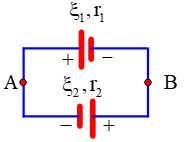
\includegraphics[width=0.2\linewidth]{../figs/PH11-FinalSem2-02-2}
\end{center}
\begin{mcq}(4)
	\item $\SI{0.3}{\ampere}$ và $\SI{1.5}{\volt}$.
	\item $\SI{1.5}{\ampere}$ và $\SI{1.5}{\volt}$.
	\item $\SI{1.5}{\ampere}$ và $\SI{0}{\volt}$.
	\item $\SI{3.0}{\ampere}$ và $\SI{0}{\volt}$.
\end{mcq}
\hideall{
\textbf{Đáp án C.}\\
Cường độ dòng điện qua mạch:
$$I=\dfrac{\calE_1+\calE_2}{r_1+r_2}=\SI{1.5}{\ampere}.$$
Hiệu điện thế giữa hai điểm A và B:
$$U_\text{AB}=\calE_1-Ir_1=\SI{0}{\volt}.$$
}

\item Một điện trở $R=\SI{4}{\ohm}$ mắc vào nguồn có suất điện động $\calE=\SI{4.5}{\volt}$ tạo thành mạch kín thì công suất toả nhiệt trên điện trở $R$ là $\calP=\SI{2.25}{\watt}$. Điện trở trong của nguồn và hiệu điện thế giữa hai đầu điện trở $R$ là
\begin{mcq}(4)
	\item $\SI{2}{\ohm}$ và $\SI{4.5}{\volt}$.
	\item $\SI{1}{\ohm}$ và $\SI{1.2}{\volt}$.
	\item $\SI{1}{\ohm}$ và $\SI{3}{\volt}$.
	\item $\SI{2}{\ohm}$ và $\SI{3}{\volt}$.
\end{mcq}
\hideall{
\textbf{Đáp án D.}\\
$$\calP_R=\dfrac{\calE^2 R}{\left(R+r\right)}\Leftrightarrow 2,25=\dfrac{4,5^2\cdot4}{\left(r+4\right)^2}\Rightarrow r=\SI{2}{\ohm}.$$
Hiệu điện thế giữa hai đầu điện trở $R$:
$$U_R=\sqrt{\calP_RR}=\SI{3}{\ohm}.$$
}

\item Hai bóng đèn sợi đốt có công suất lần lượt là $\calP_1<\calP_2$ đều làm việc bình thường ở hiệu điện thế $U$. Biểu thức so sánh đúng cường độ dòng điện và điện trở hai đèn là
\begin{mcq}(2)
	\item $I_1<I_2$ và $R_1>R_2$.
	\item $I_1>I_2$ và $R_1>R_2$.
	\item $I_1>I_2$ và $R_1<R_2$.
	\item $I_1<I_2$ và $R_1<R_2$.
\end{mcq}
\hideall{
\textbf{Đáp án A.}\\
Vì $\calP_1<\calP_2$ mà $U_1=U_2\Rightarrow I_1<I_2$ và $R_1>R_2$.
}
\end{enumerate}
\section{Câu trắc nghiệm đúng sai.} 
\textit{Thí sinh trả lời từ câu 1 đến câu 4. Trong mỗi ý \textbf{a)}, \textbf{b)}, \textbf{c)}, \textbf{d)} ở mỗi câu, thí sinh chọn đúng hoặc sai.}
\begin{enumerate}[label=\bfseries Câu \arabic*:]
	\item Khoảng cách trung bình giữa electron và proton trong nguyên tử hydrogen là $\SI{5.3E-11}{\meter}$. Cho điện tích nguyên tố $e=\SI{1.6E-19}{\coulomb}$, $m_e=\SI{9.1E-31}{\kilogram}$, $m_p=\SI{1.67e-27}{\kilogram}$, hằng số hấp dẫn $G=\SI{6.67e-11}{\newton\meter^2/\kilogram^2}$.
	\begin{center}
		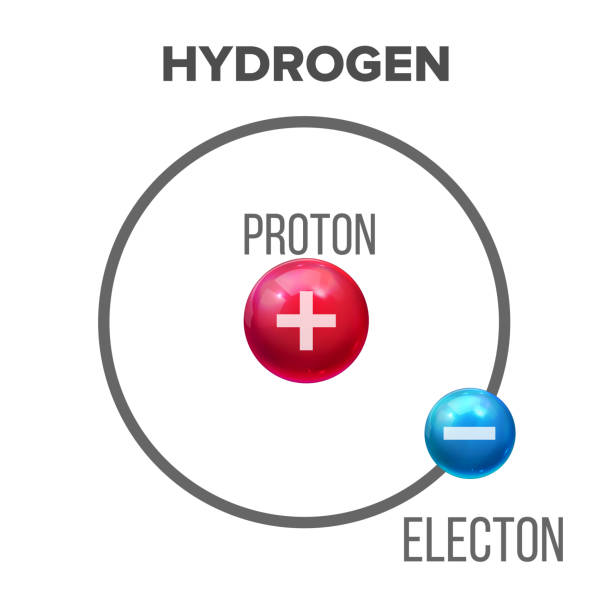
\includegraphics[width=0.25\linewidth]{../figs/PH11-FinalSem2-02-5}
	\end{center}
	\begin{enumerate}[label=\alph*)]
		\item Độ lớn lực tĩnh điện giữa electron và proton là $\SI{8.2E-8}{\newton}$.
		\item Lực hấp dẫn giữa electron và proton được xác định bằng biểu thức $F_g=G\dfrac{m_em_p}{r^2}$.
		\item Tỉ số lực điện và lực hấp dẫn là 2,3.
		\item Lực điện gây nên gia tốc $\SI{4.9E19}{\meter/\second^2}$ cho electron.
	\end{enumerate}
\hideall{
\begin{enumerate}[label=\alph*)]
	\item Đúng. Độ lớn lực tương tác tĩnh điện giữa electron và proton $F=\dfrac{ke^2}{r^2}\approx\SI{8.2E-8}{\newton}.$
	\item Đúng.
	\item Sai. 
	$$\dfrac{F_e}{F_g}=\SI{2.3E39}{}.$$
	\item Sai.
	$$a=\dfrac{F_e}{m_e}=\SI{9E22}{\meter/\second^2}.$$
\end{enumerate}
}

	\item Nhận định các phát biểu dưới đây:
	\begin{enumerate}[label=\alph*)]
		\item Dòng điện không đổi là dòng điện một chiều.
		\item Sự xuất hiện lực lạ tác động lên các điện tích bên trong nguồn là kết quả của sự chênh lệch điện thế giữa hai cực của nguồn.
		\item Với các loại nguồn điện khác nhau, lực lạ có bản chất khác nhau.
		\item Sau một thời gian sử dụng pin, cường độ dòng điện qua mạch giảm dần là do sự tăng điện trở trong của pin.
	\end{enumerate}
\hideall{
\begin{enumerate}
	\item Sai. Dòng điện không đổi là dòng điện có chiều và cường độ không đổi. Dòng điện một chiều là dòng điện có chiều không đổi. Do đó, không phải dòng điện một chiều nào cũng là dòng điện không đổi.
	\item Sai. Bản chất lực lạ không phải là lực tĩnh điện.
	\item Đúng.
	\item Đúng.
\end{enumerate}
}
	\item Cho mạch điện có sơ đồ như hình vẽ, trong đó: nguồn điện có suất điện động $\xi=\SI{12}{\volt}$, điện trở trong $r=\SI{0.4}{\ohm}$ và các điện trở mạch ngoài có giá trị $R_1=\SI{4}{\ohm}$; $R_2=\SI{6}{\ohm}$; $R_3=\SI{3}{\ohm}$; $R_4=\SI{2}{\ohm}$; điện trở ampere kế rất nhỏ.
	\begin{center}
		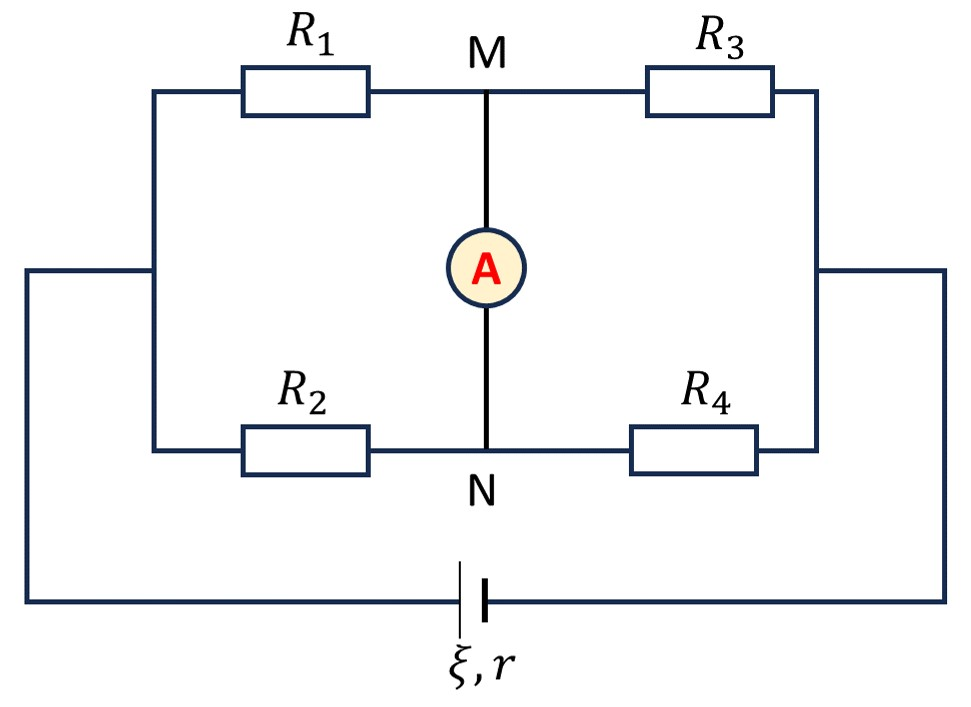
\includegraphics[width=0.5\linewidth]{../figs/PH11-FinalSem2-02-4}
	\end{center}
\begin{enumerate}[label=\alph*)]
	\item Cường độ dòng điện qua nguồn là $\SI{3.33}{\ampere}$.
	\item Dòng điện qua ampere kế có chiều từ M qua N.
	\item Cường độ dòng điện qua ampere kế là $\SI{0.6}{\ampere}$.
	\item Hiệu suất của nguồn điện là $\SI{90}{\percent}$.
\end{enumerate}
\hideall{
\begin{enumerate}[label=\alph*)]
	\item Sai. Cường độ dòng điện qua nguồn là $\SI{3}{\ampere}$.
	\item Đúng. Vì $I_1=\SI{1.8}{\ampere}>I_3=\SI{1.2}{\ampere}$.
	\item Đúng. $I_A=I_1-I_3=\SI{0.6}{\ampere}$.
	\item  Đúng. Hiệu suất nguồn điện $H=\dfrac{R_N}{r+R_N}\cdot\SI{100}{\percent}=\SI{90}{\percent}$.
\end{enumerate}
}
	\item Giả sử chiều dài của sợi trục (axon) khoảng $\SI{0.10}{\meter}$ bị kích thích bởi điện thế hoạt động. Điện thế hoạt động là cơ sở điện hóa cho các quá trình xử lý thông tin trong hệ thần kinh, bước đầu tiến tới hình thành nhận thức và tư duy. Ở trạng thái nghỉ, mặt ngoài của màng sợi trục tích điện dương bởi các ion $\ce{K^+}$ và mặt trong tích điện cùng độ lớn nhưng ngược dấu với mặt ngoài bởi các ion hữu cơ âm như hình bên dưới. Để thuận tiện cho quá trình khảo sát, có thể xem mô hình màng sợi trục như một tụ điện phẳng, điện dung $C=\dfrac{\varepsilon S}{4\pi k d}$ với các dữ liệu như sau: độ dày của màng $d=\SI{1.0E-8}{\meter}$, bán kính sợi trục $r=\SI{1.0E1}{\micro\meter}$, hằng số điện môi của màng $\varepsilon=3,0$ và $k=\SI{9E9}{\dfrac{\newton\meter^2}{\coulomb^2}}$. Điện thế hoạt động (hiệu điện thế giữa bên ngoài và bên trong màng) là $\SI{7.0E-2}{\volt}$.
	\begin{center}
		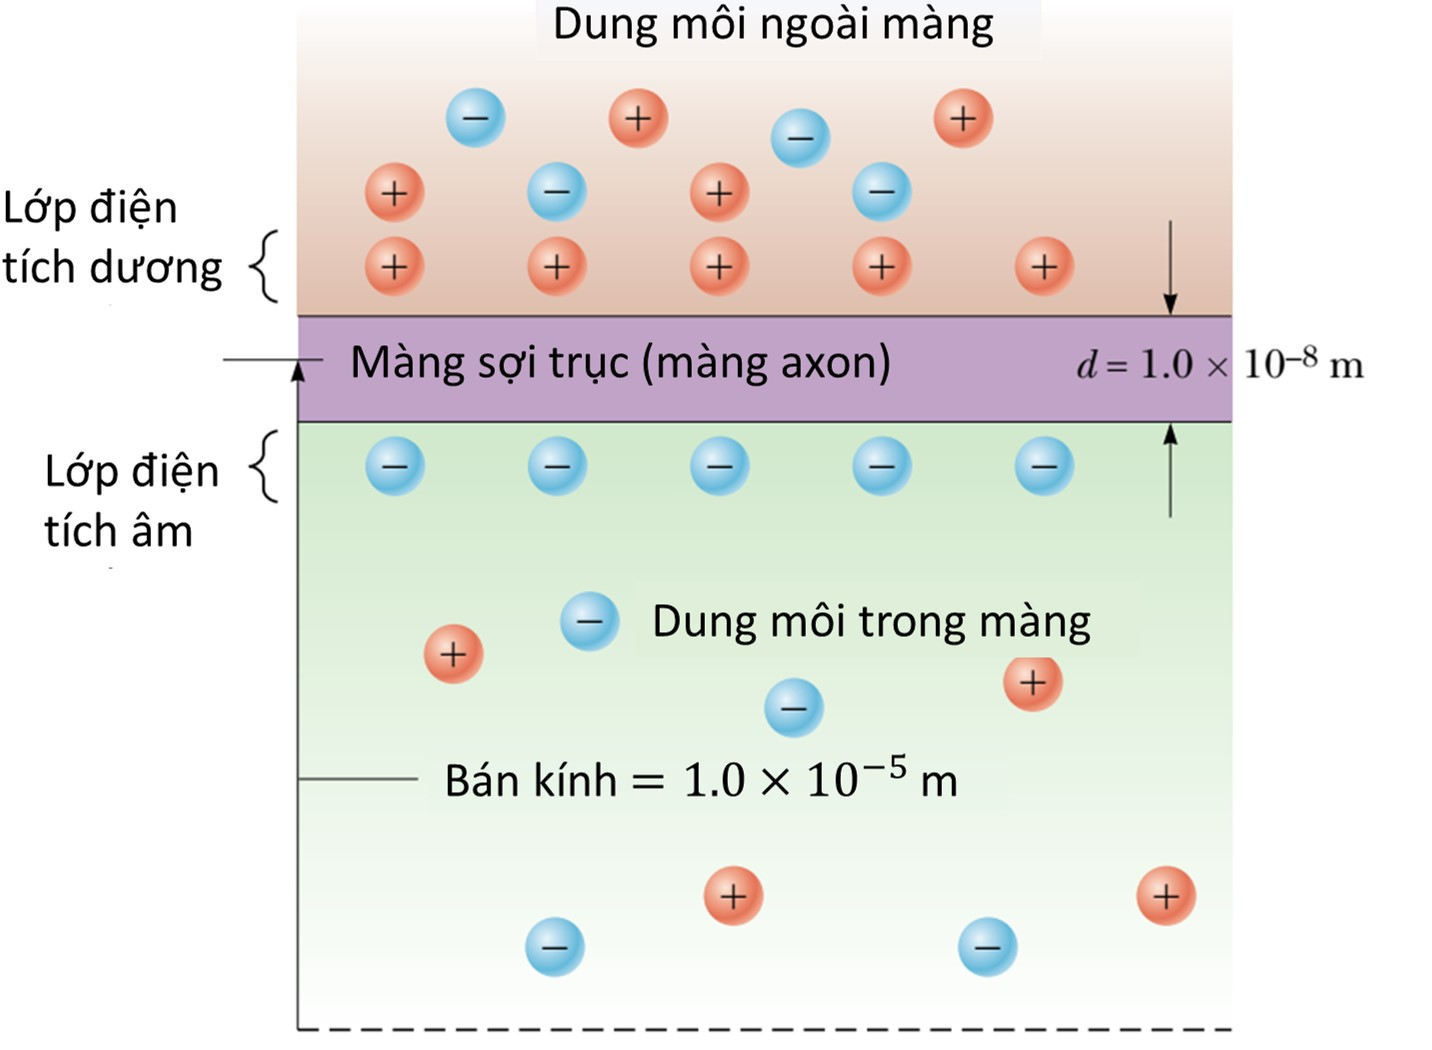
\includegraphics[width=0.55\linewidth]{../figs/PH11-FinalSem2-02-1}
	\end{center}
\begin{enumerate}[label=\alph*)]
	\item Điện trường trong màng hướng từ trong ra ngoài màng.
	\item Điện dung của màng sợi trục theo mô hình trên là $\SI{16.67}{\nano\farad}$.
	\item Số ion $\ce{K^+}$ trên bề mặt màng là $\SI{7.3E9}{}$ ion.
	\item Khi tăng điện thế giữa lớp bên trong và lớp bên ngoài từ $\SI{-7E-2}{\volt}$ lên $\SI{+3E-2}{\volt}$ thì điện lượng dịch chuyển qua màng là $\SI{6.7E-10}{\coulomb}$.
\end{enumerate}
\hideall{
\begin{enumerate}[label=\alph*)]
	\item Sai. Điện trường hướng từ ngoài màng vào trong.
	\item Đúng. Diện tích bề mặt của màng là diện tích mặt trụ bán kính $r$ chiều dài $\ell=\SI{0.1}{\meter}$: $S=2\pi r\ell$.
	\\Điện dung:
	$$C=\dfrac{\varepsilon S}{4\pi kd}=\dfrac{\varepsilon \cdot2\pi r\ell}{4\pi k d}=\dfrac{3\cdot\left(\SI{E-5}{\meter}\right)\cdot\left(\SI{0.1}{\meter}\right)}{2\cdot\left(\SI{9E9}{\dfrac{\newton\meter^2}{\coulomb^2}}\right)\cdot\left(\SI{E-8}{\meter}\right)}\approx\SI{16.67}{\nano\farad}.$$
	\item Đúng. Điện tích trên màng dưới điện áp $\SI{7.0E-2}{\volt}$:
	$$Q=CU\approx\SI{1.167}{\nano\coulomb}.$$
	Số ion $\ce{K^+}$ trên màng:
	$$N=\dfrac{Q}{e}\approx\SI{7.3E9}{\text{ion}}.$$
	\item Sai.\\
	Điện tích trên màng lúc đầu:
	$$Q_1=CU_1\approx\SI{-1.167}{\nano\coulomb}.$$
	Điện tích trên màng lúc sau:
	$$Q_2=CU_2\approx\SI{0.5}{\nano\coulomb}.$$
	Điện lượng dịch chuyển qua màng:
	$$\Delta Q=\left|Q_2-Q_1\right|=\SI{1.667}{\nano\coulomb}.$$
\end{enumerate}
}
\end{enumerate}
\section{Câu trắc nghiệm trả lời ngắn.} \textit{Thí sinh trả lời từ câu 1 đến câu 6.}
\begin{enumerate}[label=\bfseries Câu \arabic*:]
	\item Một hạt bụi đang cân bằng lơ lửng trong một điện trường đều giữa hai bản kim loại phẳng, tích điện trái dấu đặt nằm ngang. Biết hạt bụi có khối lượng $\SI{100}{\milli\gram}$ và mang điện tích $\SI{-2E-6}{\volt}$, lấy $g=\SI{10}{\meter/\second^2}$. Xác định độ lớn cường độ điện trường giữa 2 bản kim loại nói trên theo đơn vị $\SI{E5}{\volt/\meter}$.
	\hideall{
Hạt bụi nằm cân bằng nên:
$$\left|q\right|E=mg\Rightarrow E=\dfrac{mg}{\left|q\right|}	=\dfrac{\left(\SI{100E-3}{\kilogram}\right)\cdot\left(\SI{10}{\meter/\second^2}\right)}{\SI{2E-6}{\coulomb}}=\SI{5E5}{\volt/\meter}.$$
}

\item Để tạo ra tia X người ta dùng một ống phóng tia X có hiệu điện thế giữa hai cực là $\SI{100}{\kilo\volt}$. Một electron khi chuyển động giữa hai cực này sẽ chịu tác dụng của lực điện trường có độ lớn $F=\SI{5E-10}{\newton}$. Khoảng cách giữa hai cực của ống phóng tia X này là bao nhiêu \textit{(tính theo đơn vị $\si{\centi\meter}$)}?
\hideall{
Cường độ điện trường trong ống tia X:
$$E=\dfrac{F}{\left|e\right|}=\SI{3.125E6}{\volt/\meter}.$$
Khoảng cách giữa hai cực của ống tia X:
$$d=\dfrac{U}{E}=\SI{0.032}{\meter}=\SI{3.2}{\centi\meter}.$$
}

\item Cho mạch điện có sơ đồ như hình vẽ. Trong đó $R$ là biến trở con chạy, $R_0$ là điện trở có giá trị không đổi và E là nam châm điện. Nam châm E hút lượng vụn sắt nhiều nhất khi con chạy của biến trở ở vị trí nào?
\begin{center}
	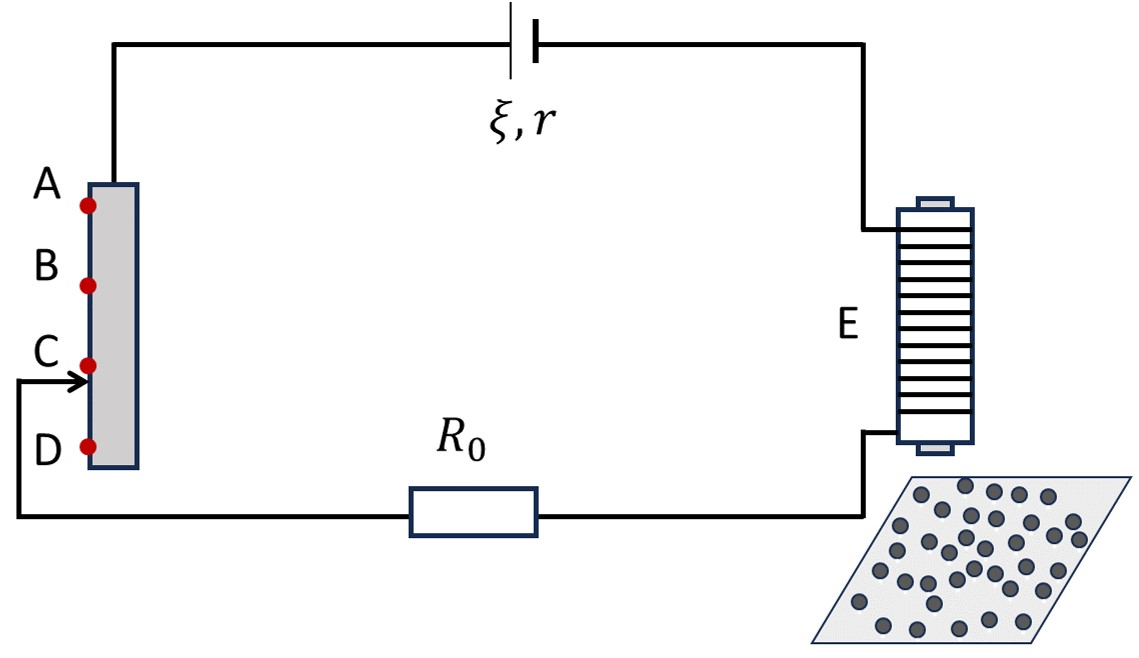
\includegraphics[width=0.6\linewidth]{../figs/PH11-FinalSem2-02-6}
\end{center}
\hideall{
Nam châm E hút sắt nhiều nhất khi cường độ dòng điện qua nam châm lớn nhất $\Leftrightarrow R_\text{min}\Rightarrow $ con chạy của biến trở ở vị trí A.
}

\item  Một dòng điện không  đổi có cường độ $\SI{10}{\ampere}$ chạy qua dây dẫn bằng kim loại, tiết diện tròn, có bán kính tiết diện $\SI{1.2}{\milli\meter}$. Biết mật độ electron tự do là $\SI{6E28}{\text{electron}/\meter^3}$. Xác định tốc độ dịch chuyển có hướng của các electron trong dây dẫn theo đơn vị $\si{\milli\meter/\second}$ \textit{(làm tròn đến 2 chữ số thập phân)}.
\hideall{
$v=\dfrac{I}{\pi r^2ne}=\SI{0.23}{\milli\meter/\second}$.
}

\item Giả sử phòng bạn Minh có 4 bóng đèn loại $\SI{25}{\watt}$, 1 tủ lạnh $\SI{120}{\watt}$, 1 máy lạnh loại $\SI{750}{\watt}$. Bình quân mỗi ngày các thiết bị hoạt động 5 giờ, mỗi tháng là 30 ngày, giá tiền điện là $\SI{3500}{\text{đồng}/\kilo\watt\hour}$ thì mỗi tháng bạn Minh phải trả bao nhiêu tiền?
\hideall{
$\SI{509250}{\text{đồng}}.$
}
	\item Cho mạch điện có sơ đồ như hình vẽ: các điện trở giống nhau, hai nguồn điện giống nhau có cùng điện trở trong $\SI{1}{\ohm}$, ampere kế có điện trở không đáng kể và volt kế có điện trở rất lớn. Biết ampere kế chỉ $\SI{1.0}{\ampere}$ và volt kế chỉ $\SI{4.5}{\volt}$. Tìm suất điện động của nguồn điện theo đơn vị volt $\left(\si{\volt}\right)$.
	\begin{center}
		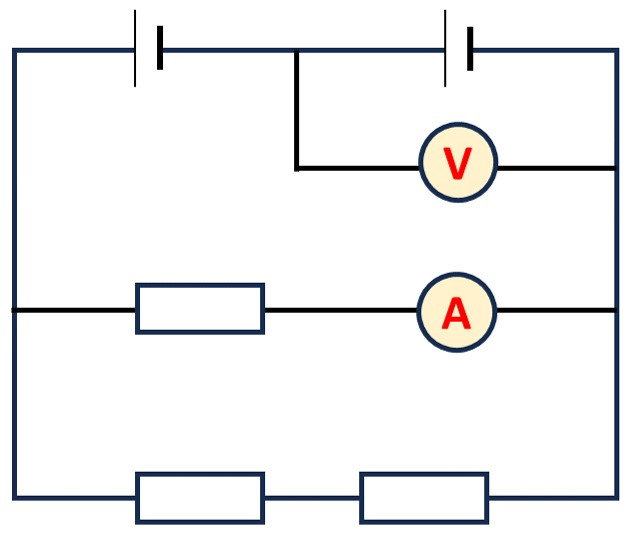
\includegraphics[width=0.35\linewidth]{../figs/PH11-FinalSem2-02-3}
	\end{center}
	\hideall{
Cường độ dòng điện mạch chính:
$$I=1+\dfrac{1\cdot R}{2R}=\SI{1.5}{\ampere}.$$
Suất điện động của nguồn:
$$\calE=U_V+Ir=\SI{4.5}{\volt}+\left(\SI{1.5}{\ampere}\right)\cdot\left(\SI{1}{\ohm}\right)=\SI{6}{\volt}.$$	
}
\end{enumerate}
\begin{center}
	\textbf{--- HẾT ---}
\end{center}